% !TEX program = xelatex
\documentclass[12pt,a4paper]{article}
\usepackage[T1]{fontenc}
%\usepackage{tgpagella, eulervm}

% --- XeLatex/LuaLatex ---
\usepackage[no-math]{fontspec}
\IfFontExistsTF{Fira Sans}{
	\setmainfont{Fira Sans}
}

% % --- This is for pdflatex ---
%\usepackage[light, sfdefault]{FiraSans}

\usepackage[italic]{mathastext}
\usepackage[indonesian]{babel}
\usepackage{booktabs}
\usepackage{geometry}
\usepackage{tabularx}
\usepackage{graphicx}
\usepackage{float}
\usepackage{xcolor}
\usepackage{hyperref}
\hypersetup{
	colorlinks=true,  % Colours links instead of boxes
	urlcolor=blue,    % Colour for external hyperlinks
	linkcolor=blue,   % Colour of internal links (sections, etc.)
	citecolor=red,    % Colour of citations
	bookmarks=true,   % Adds PDF bookmarks
	hypertexnames=true
}

\geometry{left=2cm, right=2cm, top=2cm}
\title{\textbf{Panduan Penggunaan Tangra}}
\author{Observatorium Bosscha}
\hyphenation{me-la-ku-kan peng-amat-an deng-an align-ment}
\begin{document}
\maketitle
\noindent\rule{\linewidth}{0.4pt}
\section*{Prasyarat}
Sebelum memulai, pastikan hal berikut sudah terpenuhi:
\begin{itemize}
\item Data video/fits sudah tersalin lengkap (tidak ada file yang hilang/korup).
\item Waktu observasi pada sistem akuisisi sudah tersinkron (NTP/GPS) dan dicatat dalam UTC.
\item Anda mengetahui mode akuisisi data (ADV atau FITS sequence) serta bit depth yang digunakan.
\item Nama target, waktu kejadian prediksi, dan durasi observasi sudah disiapkan untuk verifikasi hasil.
\end{itemize}

\section*{Instalasi}
\begin{enumerate}
	\item Unduh file instalasi Tangra dari laman Okultasi 2026 Observatorium Bosscha dan ekstrak ke folder kerja anda.
	\begin{center}
		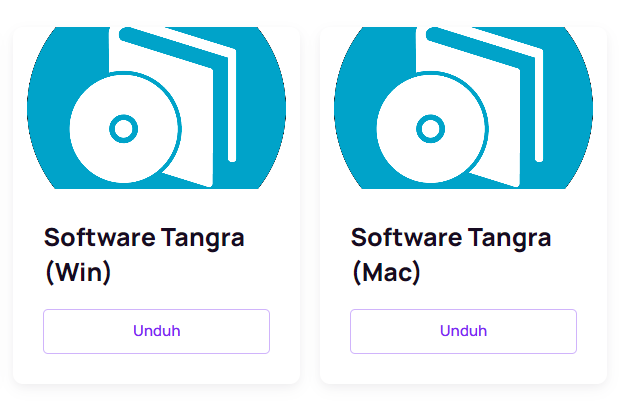
\includegraphics[width=0.35\linewidth]{tangra-download}
	\end{center}
	\item Unduh file contoh data dari laman Okultasi 2026. Ekstrak pada folder kerja, berdampingan dengan folder Tangra untuk memudahkan.
	\begin{center}
		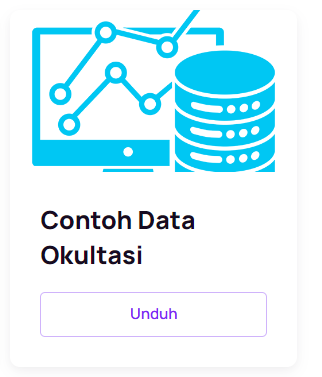
\includegraphics[width=0.2\linewidth]{tangra-data-download}
	\end{center}
	\item Klik ganda pada file \texttt{Tangra.exe} maka jendela utama Tangra akan muncul. Lakukan upgrade ke versi terbaru sebelum menggunakannya (klik pada tulisan dalam kotak merah). Tunggu sampai proses upgrade selesai.
	\begin{center}
		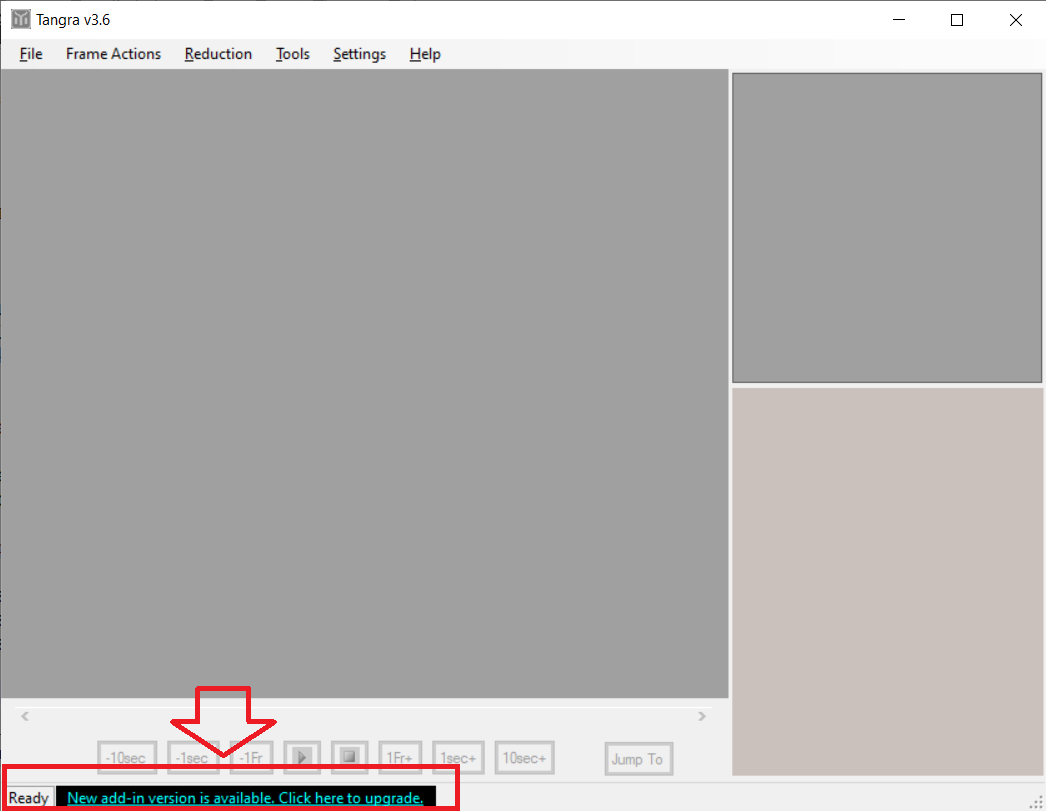
\includegraphics[width=0.5\linewidth]{tangra-upgrade}
	\end{center}
	\begin{center}
		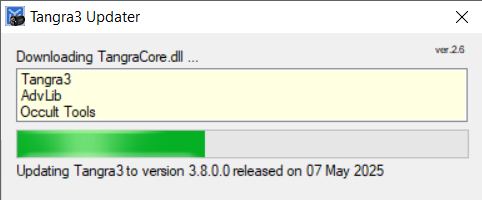
\includegraphics[width=0.5\linewidth]{tangra-upgrade-progress}
	\end{center}
\end{enumerate}

\section*{Aplikasi Ekstraksi Kurva Cahaya}
\begin{enumerate}
	\item Klik \textit{File > Open Video} untuk membuka file contoh data (ekstensi .adv). Klik OK pada jendela yang muncul (biarkan pilihan default). Maka jendela utama akan muncul dan menampilkan data.
	\begin{center}
		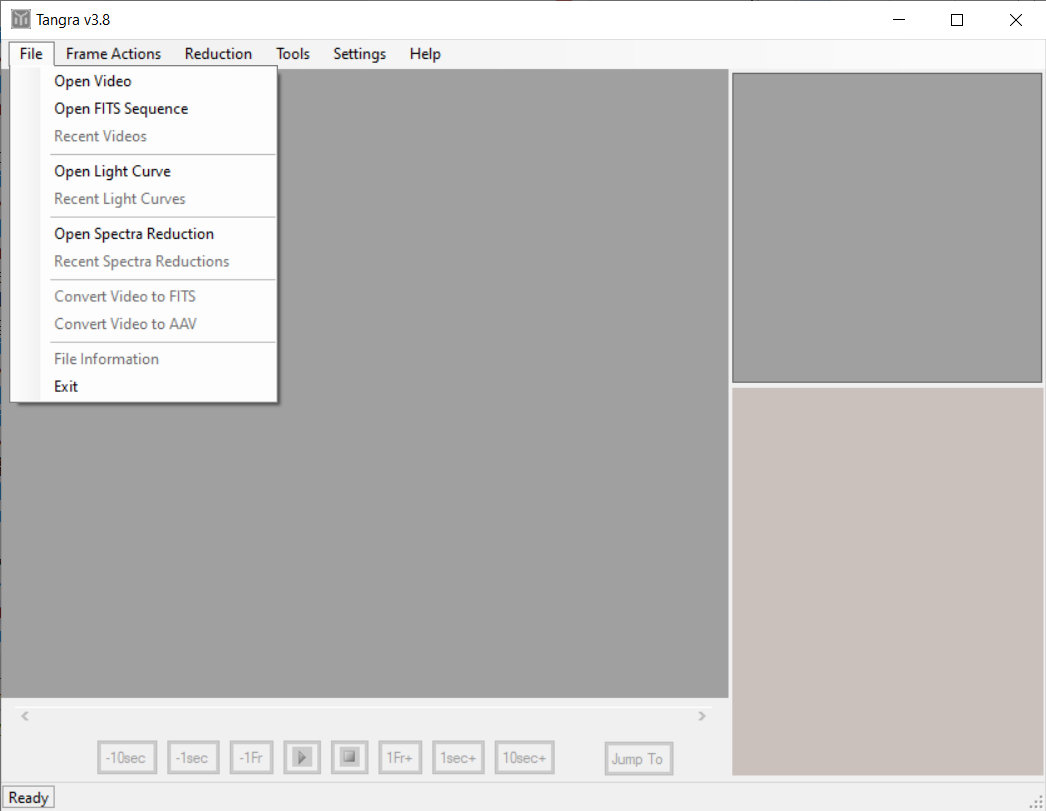
\includegraphics[width=0.5\linewidth]{tangra-opendata}
	\end{center}
	\begin{center}
		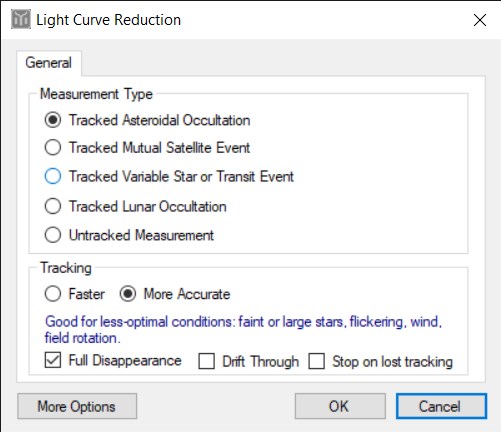
\includegraphics[width=0.3\linewidth]{tangra-lc-reduction}
	\end{center}
	\underline{Catatan:}
	Jika tampilan data di jendela utama kurang jelas, atur rentang dinamik dengan \textit{slider} yang disediakan dengan mengaksesnya seperti gambar berikut. Tekan \textbf{Close} setelah yakin dengan hasilnya.
	\begin{center}
		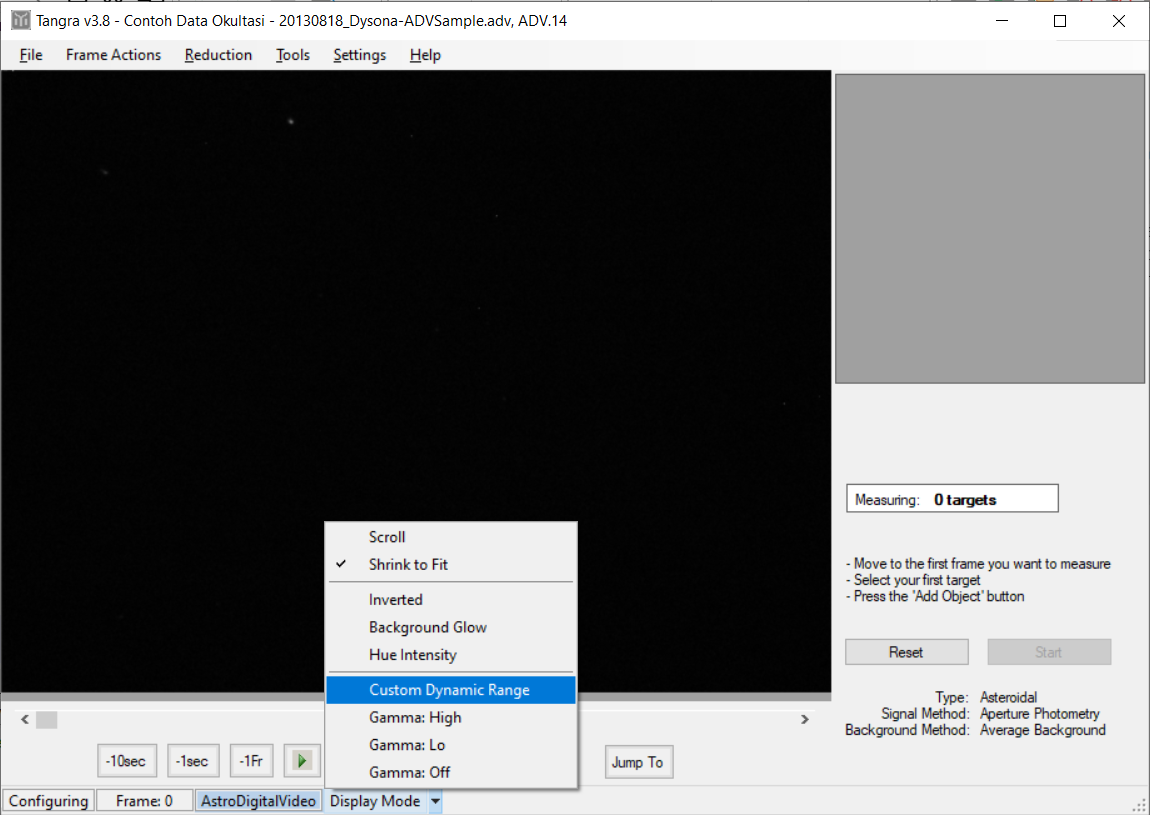
\includegraphics[width=0.4\linewidth]{tangra-main-window}
	\end{center}
	\begin{center}
		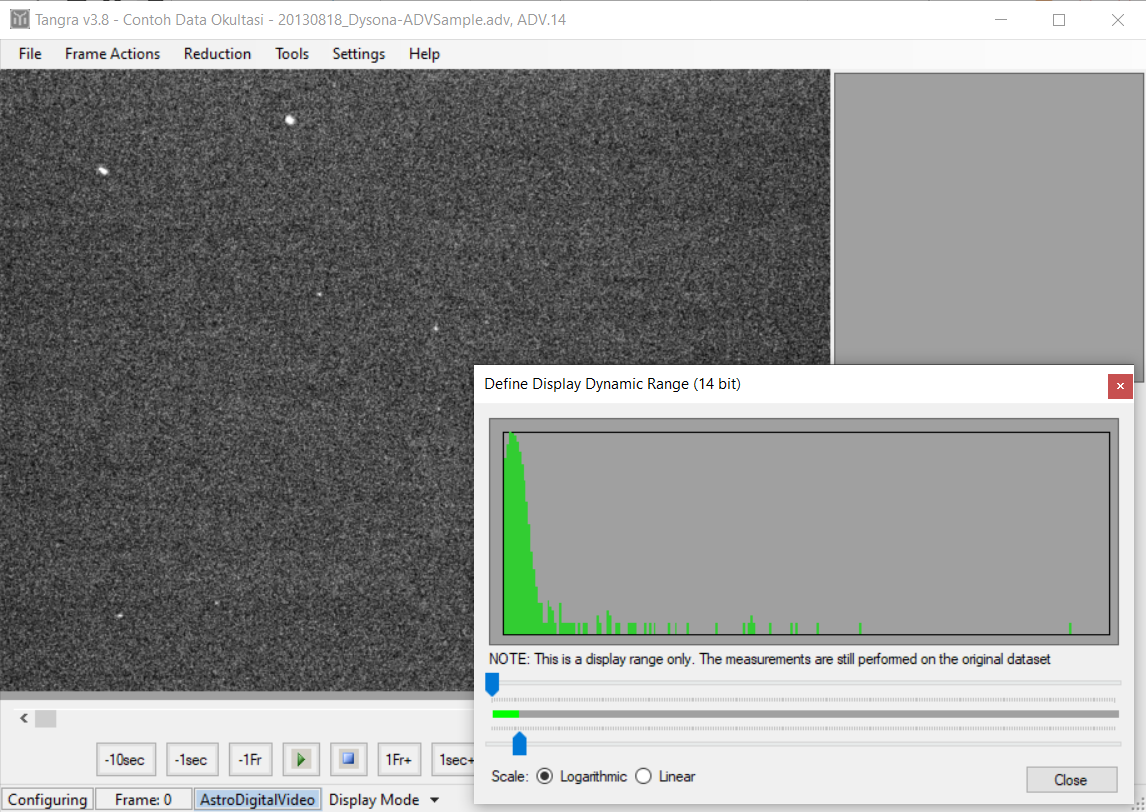
\includegraphics[width=0.4\linewidth]{tangra-dynrange2}
	\end{center}
	 
	\underline{Catatan:} 
	\begin{itemize}
		\item Jika file data berupa *.fits, buka dengan \textit{File > Open FITS Sequence}. Arahkan ke folder contoh data (tekan bagian yang ditandai panah).
		\begin{center}
			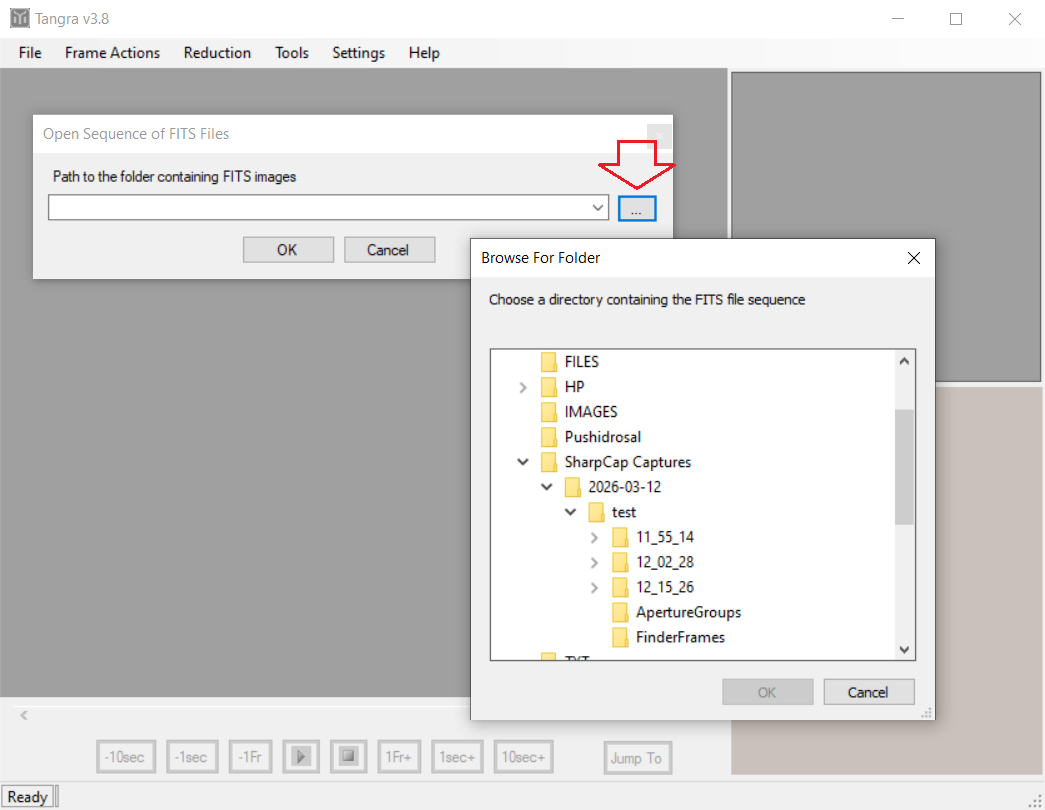
\includegraphics[width=0.4\linewidth]{tangra-open-fits}
		\end{center}
		\item Jika data diambil dengan kamera CMOS, pilih \textbf{Video}, tekan OK.
		\begin{center}
			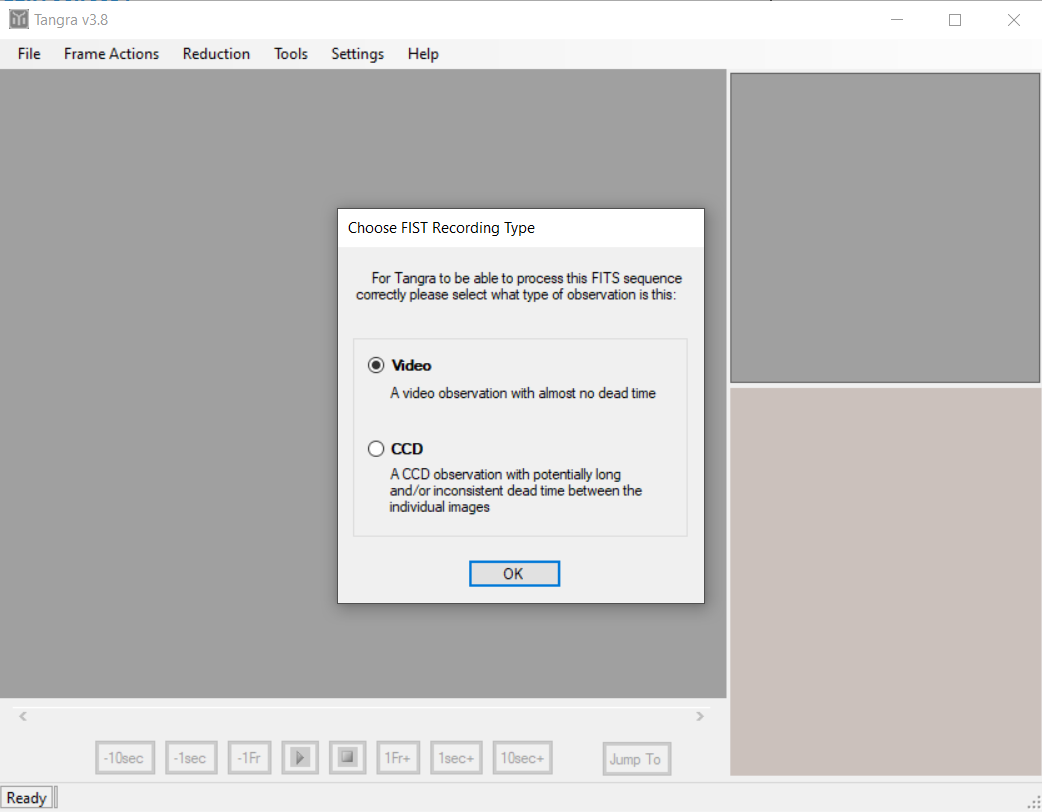
\includegraphics[width=0.4\linewidth]{tangra-open-fits-video}
		\end{center}
		\item Pada pemetaan header FITS, pilih \texttt{DATE-OBS} sebagai sumber waktu absolut \textit{frame} dan \texttt{EXPTIME} sebagai durasi paparan. Pastikan opsi waktu merepresentasikan \textbf{awal} paparan (bukan tengah/akhir paparan).
		\begin{center}
			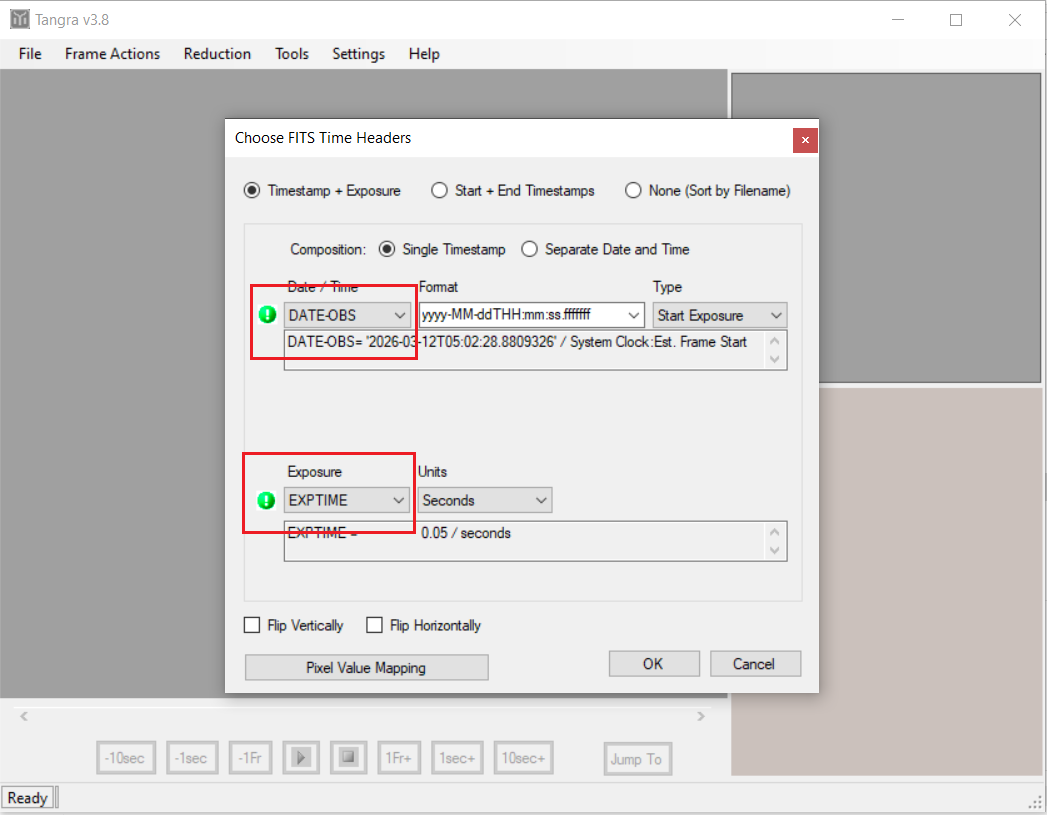
\includegraphics[width=0.4\linewidth]{tangra-open-fits-header}
		\end{center}
		\item Jika file data terdeteksi memiliki masalah akurasi \textit{timing}, akan muncul jendela koreksi. Tinjau pesannya, lalu tekan OK untuk melanjutkan.
		\begin{center}
			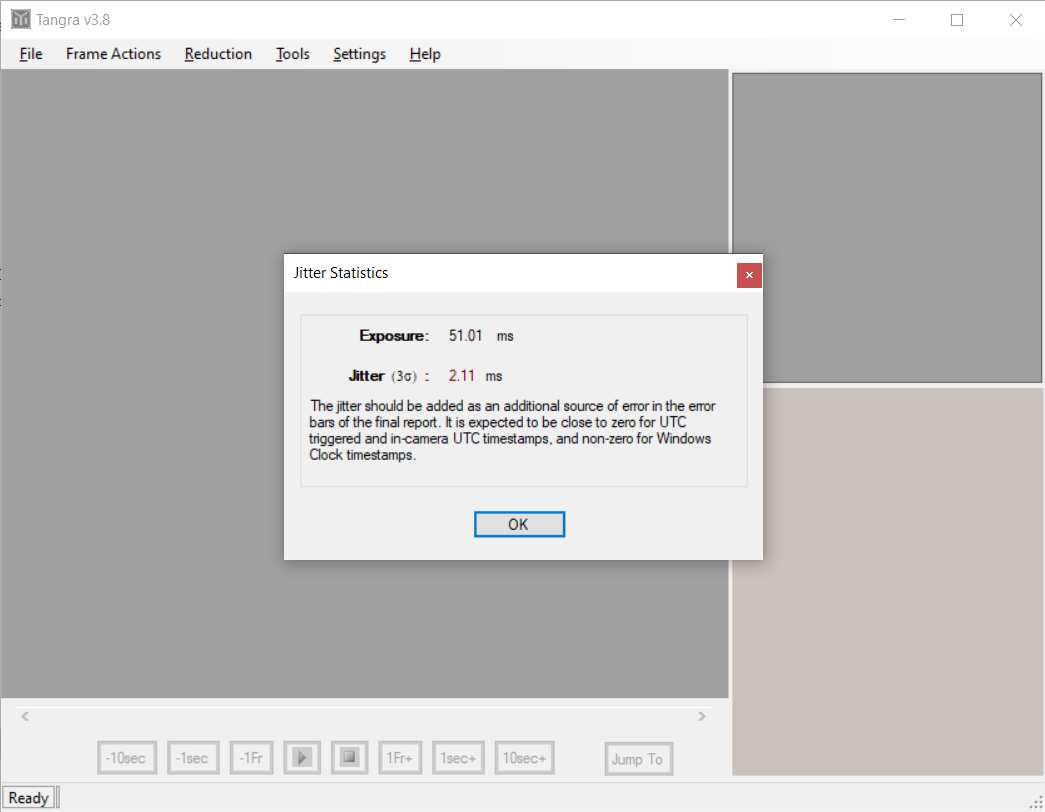
\includegraphics[width=0.4\linewidth]{tangra-open-fits-jitter}
		\end{center}
		\item Atur rentang dinamis dengan menggunakan \textit{slider} sampai obyek/bintang jelas terlihat dan tekan OK.
		\begin{center}
			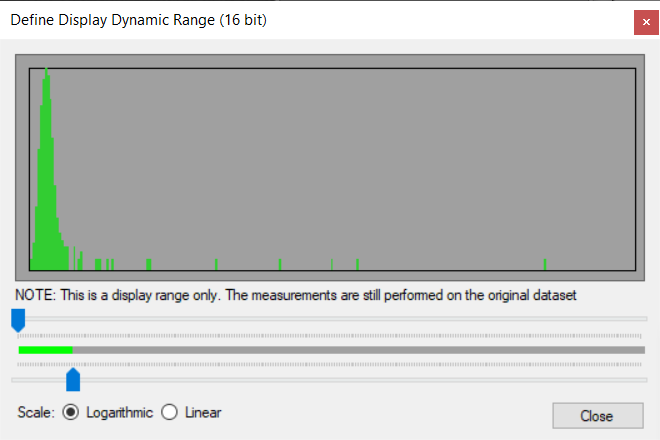
\includegraphics[width=0.4\linewidth]{tangra-dynrange}
		\end{center}
		\item Sampai di sini, prosesnya mirip dengan proses membuka file .adv. Tekan OK pada jendela berikutnya, sampai file terbuka sempurna di Tangra.
		\begin{center}
			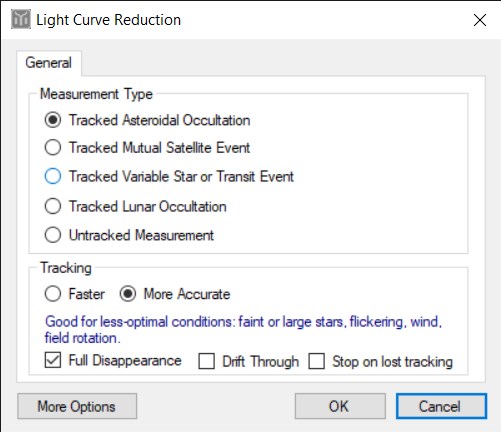
\includegraphics[width=0.4\linewidth]{tangra-lc-reduction}
		\end{center}
		\begin{center}
			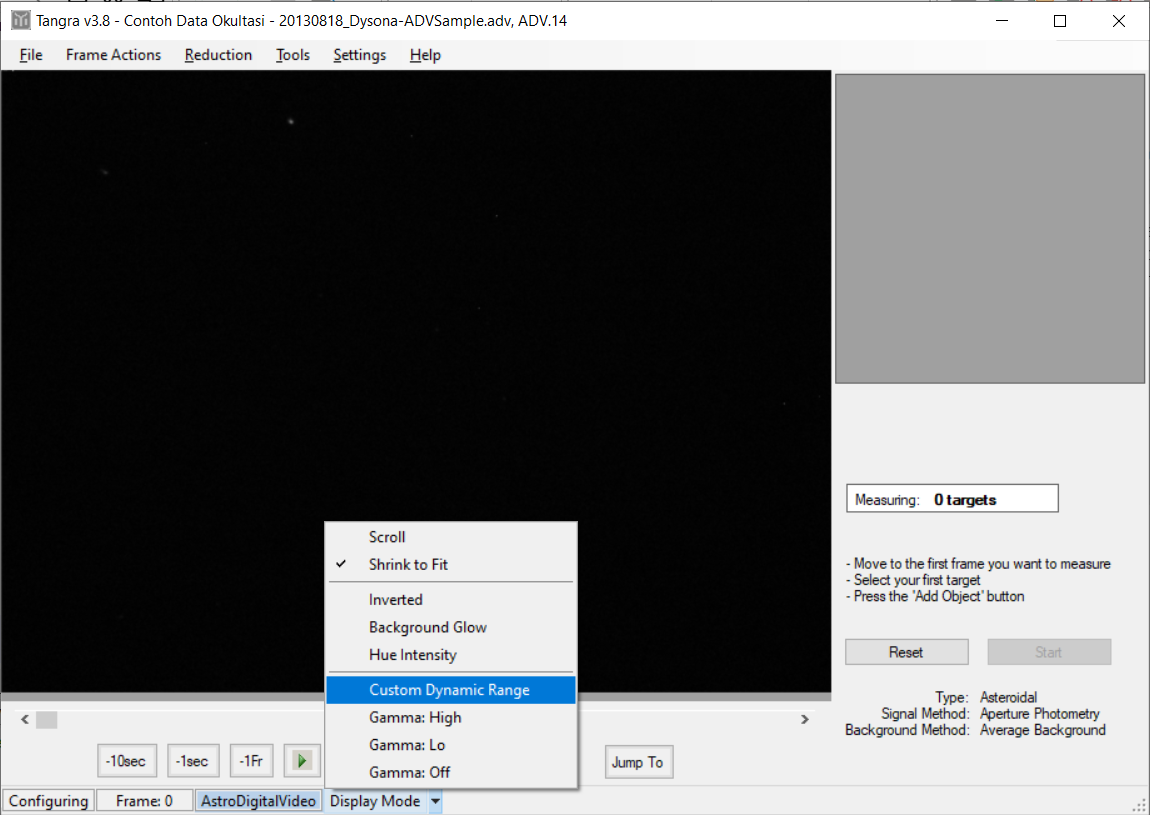
\includegraphics[width=0.4\linewidth]{tangra-main-window}
		\end{center}
	\end{itemize}
	\item Klik pada bintang target, lalu klik \textbf{Add Object}.
	\begin{center}
		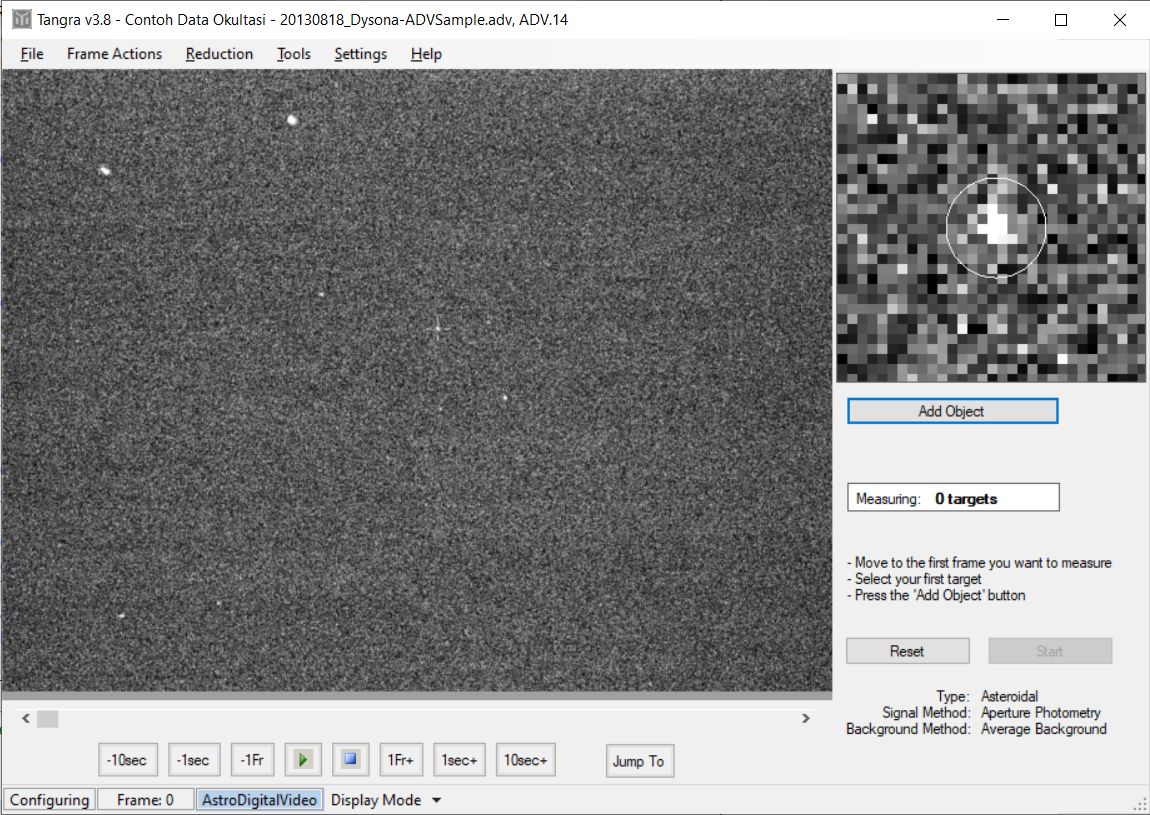
\includegraphics[width=0.4\linewidth]{tangra-add-object}
	\end{center}
	\item Pada jendela pengaturan objek target, pastikan pilihan seperti pada gambar lalu tekan \textbf{Add}. Jika medan bintang sangat minim, aktifkan \textbf{Auto tracked} untuk membantu pelacakan posisi target antar-\textit{frame}.
	\begin{center}
		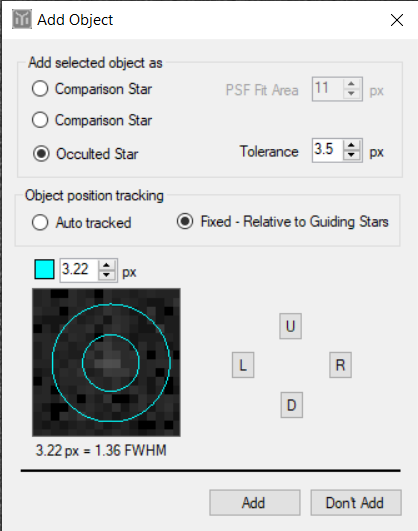
\includegraphics[width=0.4\linewidth]{tangra-add-object2}
	\end{center}
	\item Tambahkan satu atau lebih bintang lain sebagai bintang pembanding/\textit{guiding}. Pilih bintang yang stabil, tidak jenuh, dan tidak terlalu dekat tepi citra. Pastikan \textit{setting} seperti pada gambar lalu tekan \textbf{Add}.
	\begin{center}
		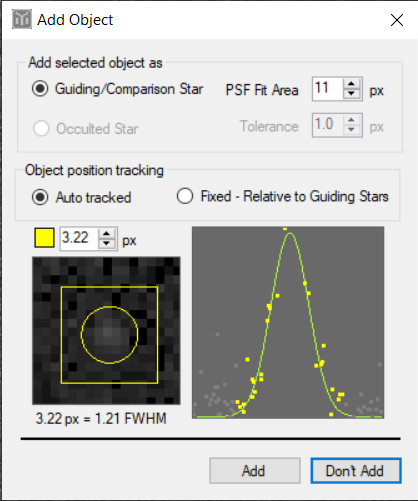
\includegraphics[width=0.4\linewidth]{tangra-add-comp}
	\end{center}
	\underline{Catatan:} Jika diperlukan, atur aperture untuk masing--masing bintang secara terpisah (bisa juga menggunakan aperture yang sama untuk semua bintang, sesuaikan dengan data yang dimiliki) dengan klik \textbf{Adjust}. Tekan OK jika sudah.
	\begin{center}
		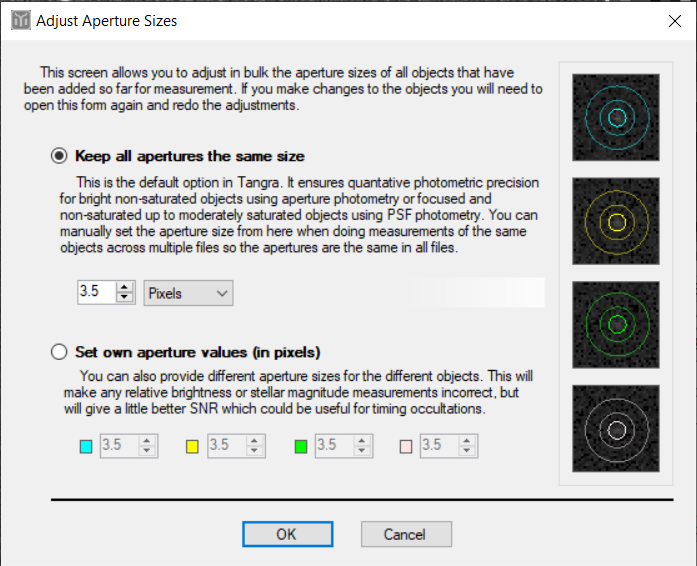
\includegraphics[width=0.5\linewidth]{tangra-adjust}
	\end{center}
	\item Tekan \textbf{Start} untuk memulai ekstraksi data. Setelahnya, jendela baru akan muncul dan menampilkan kurva cahaya masing--masing bintang.
	\begin{center}
		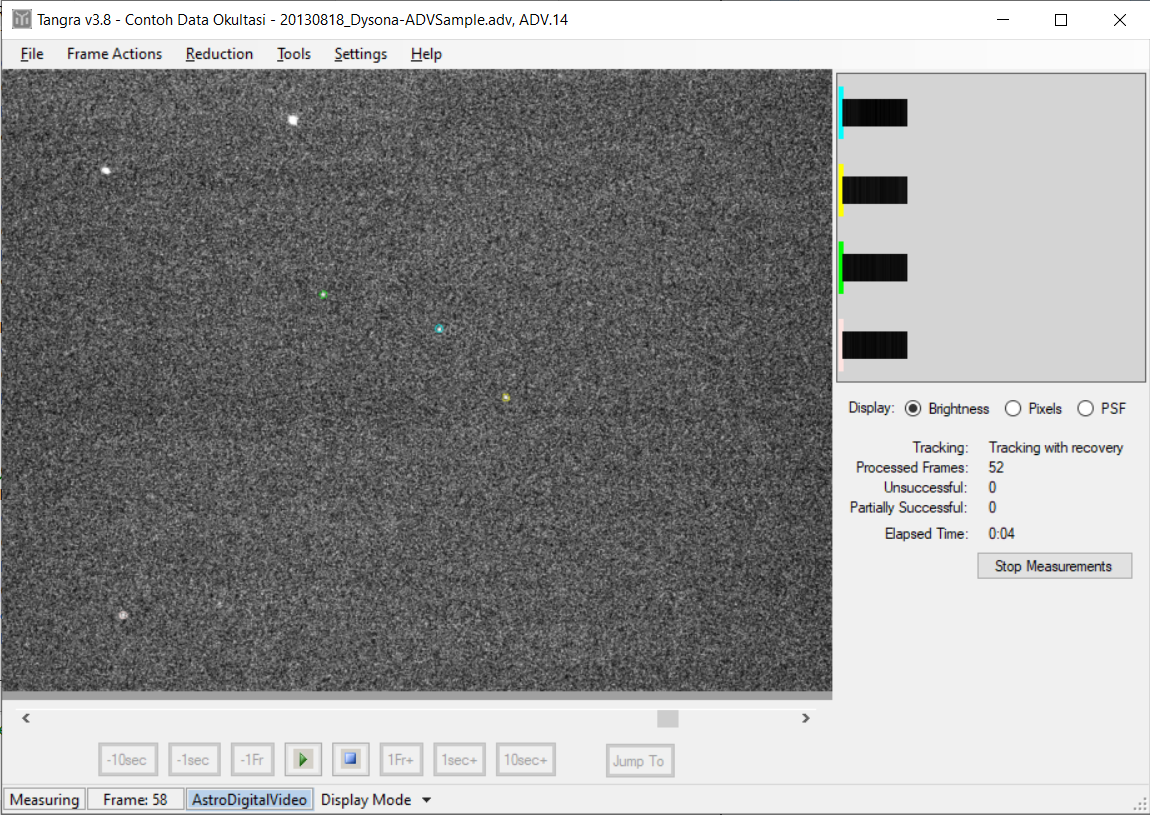
\includegraphics[width=0.5\linewidth]{tangra-start-extract}
	\end{center} 
	\begin{center}
		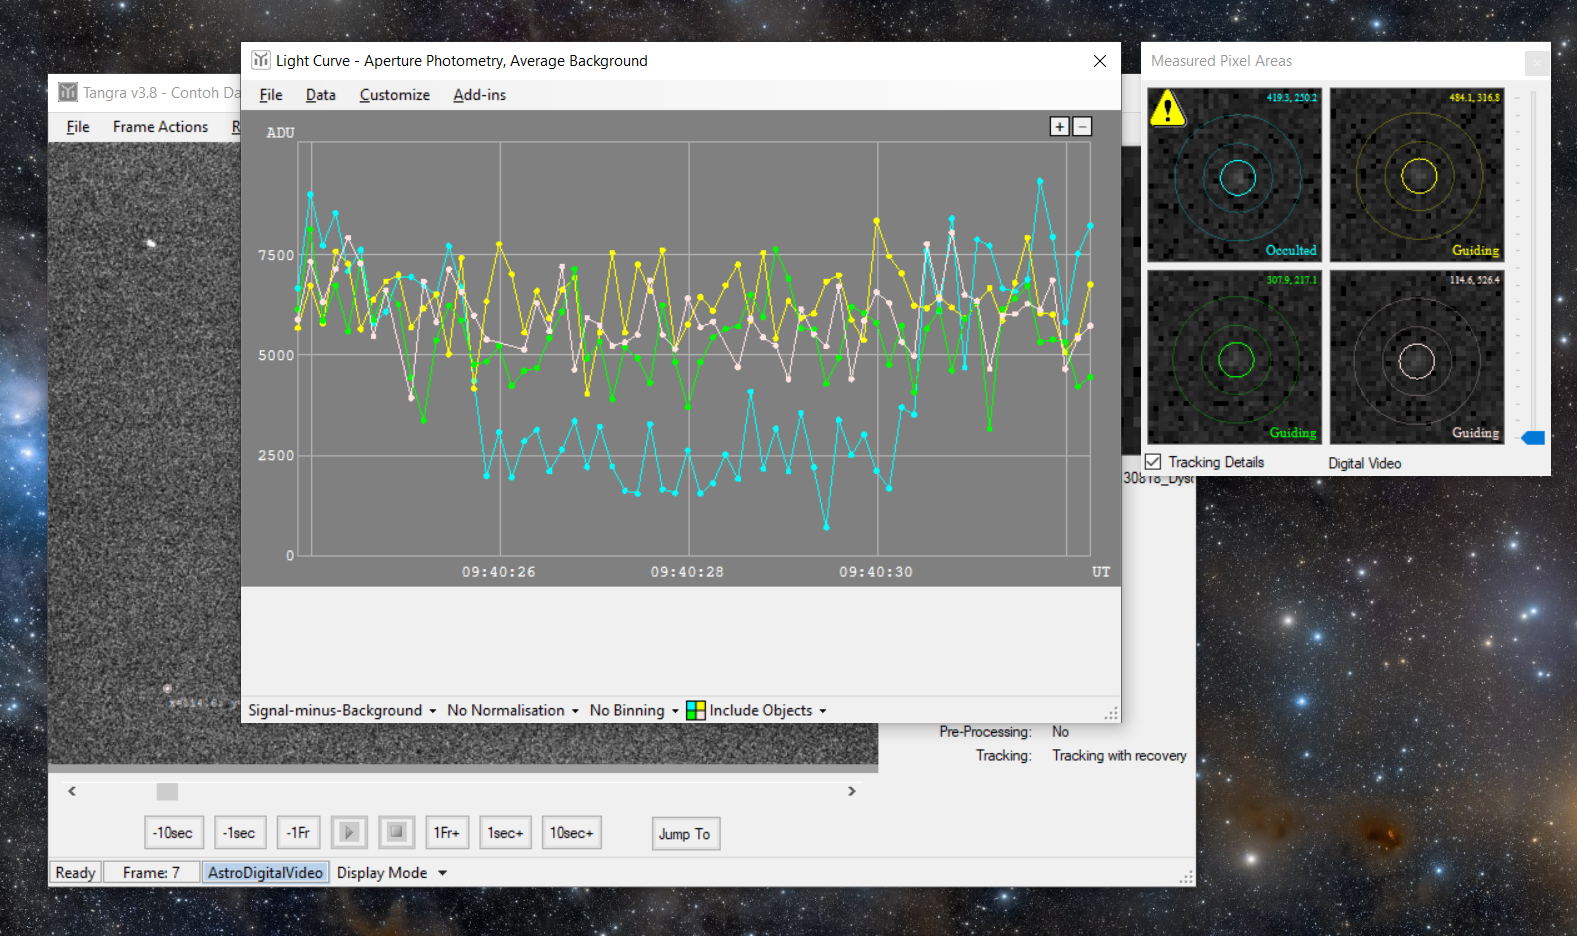
\includegraphics[width=0.5\linewidth]{tangra-hasil}
	\end{center} 
	\item Kurva cahaya yang ditampilkan dapat dikustomisasi dengan memilih bintang--bintang yang relevan (opsional).
	\begin{center}
		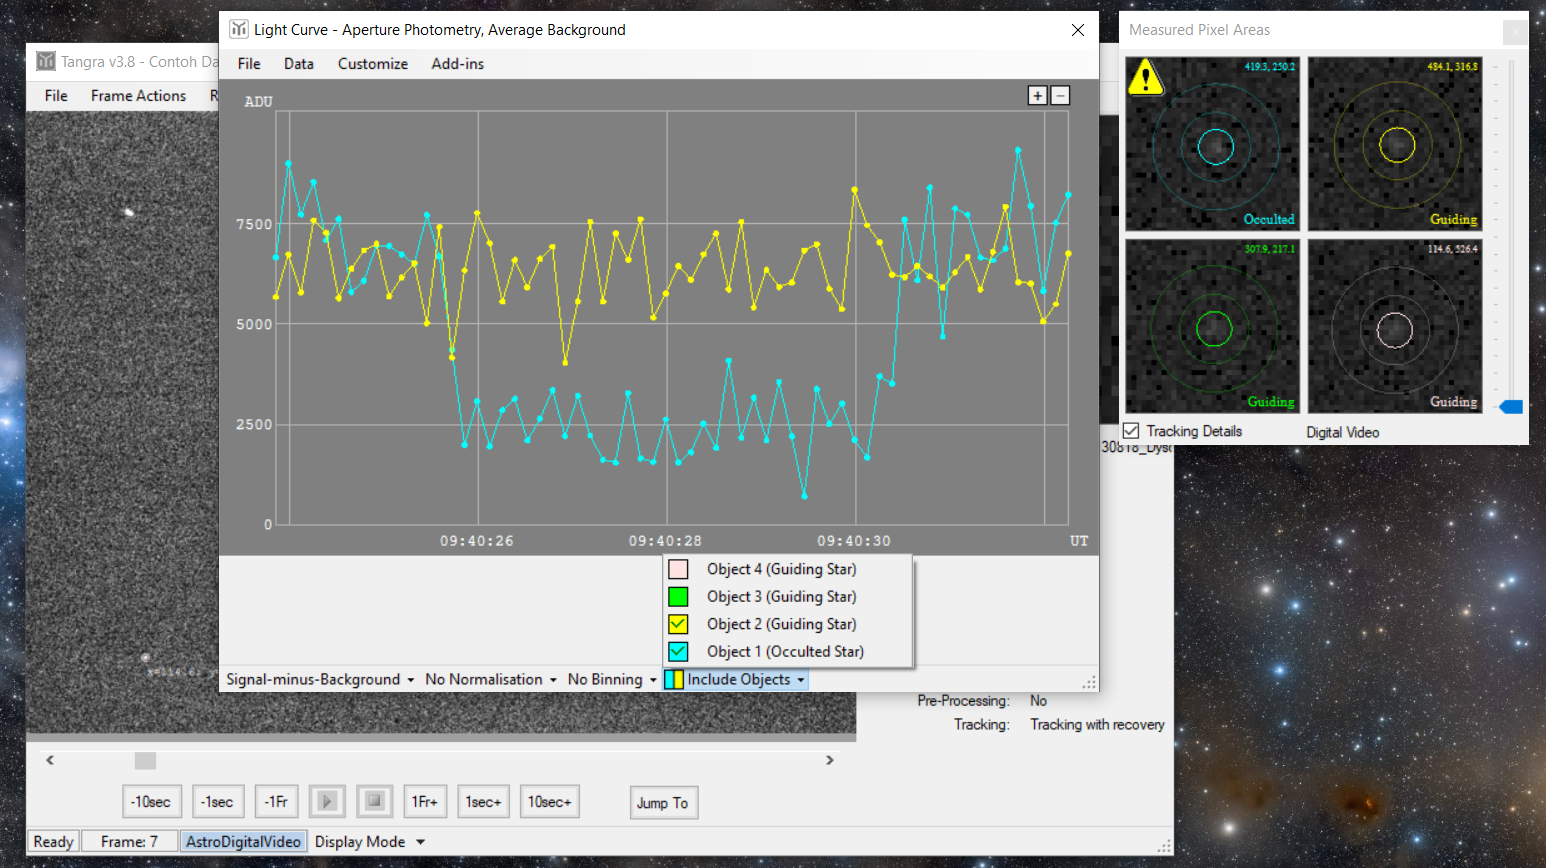
\includegraphics[width=0.5\linewidth]{tangra-hasil-pilih}
	\end{center}
	\underline{Catatan:}
	Pilih \textit{Data > Quick Re-process} untuk mencoba beberapa pilihan (lihat kotak merah) untuk mendapatkan hasil terbaik.
	\begin{center}
		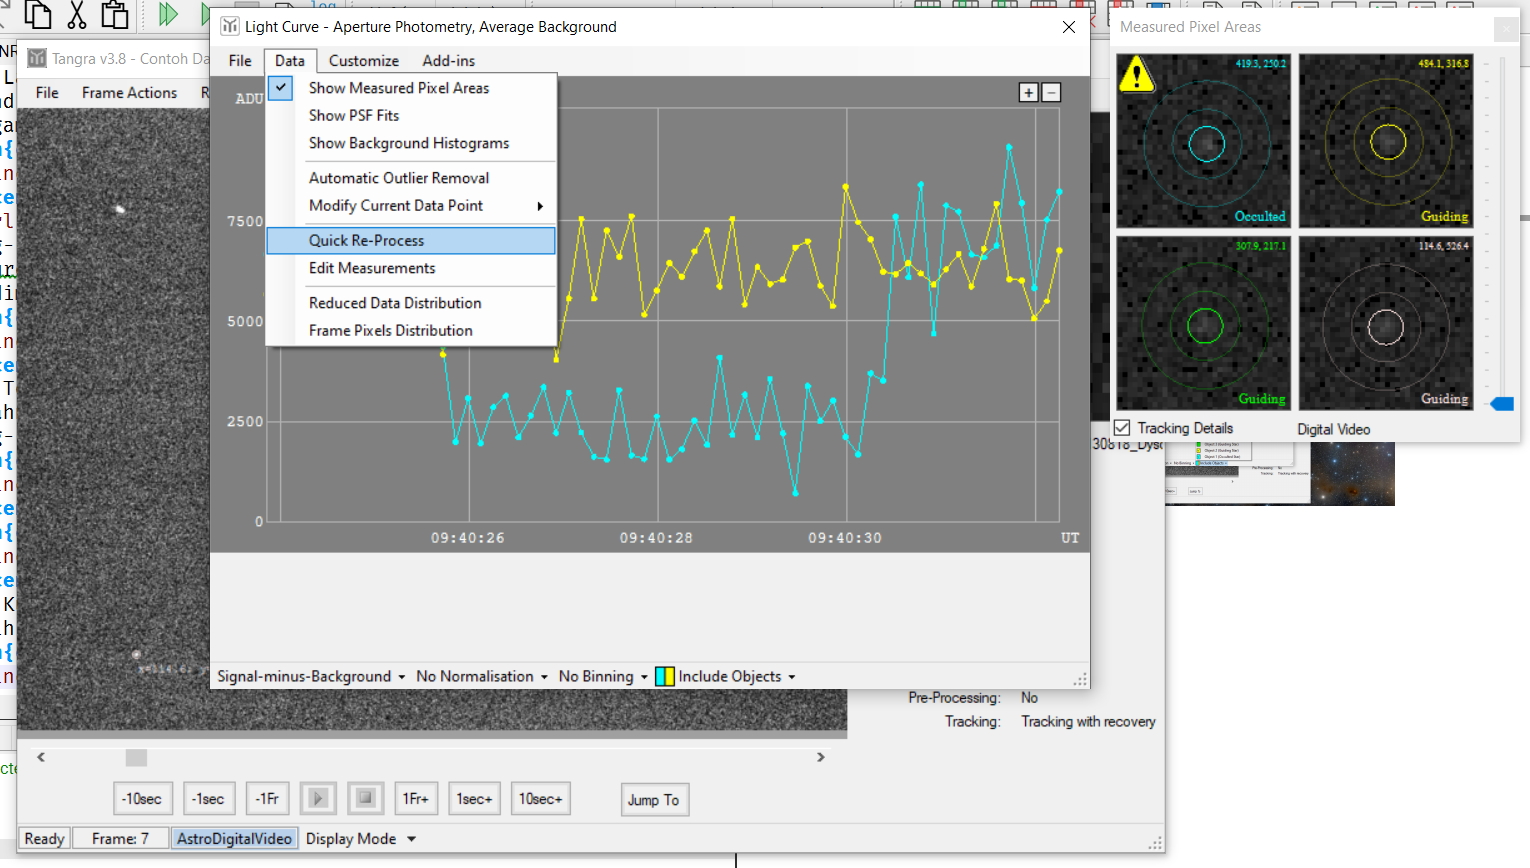
\includegraphics[width=0.5\linewidth]{tangra-reprocess}
	\end{center}
	\begin{center}
		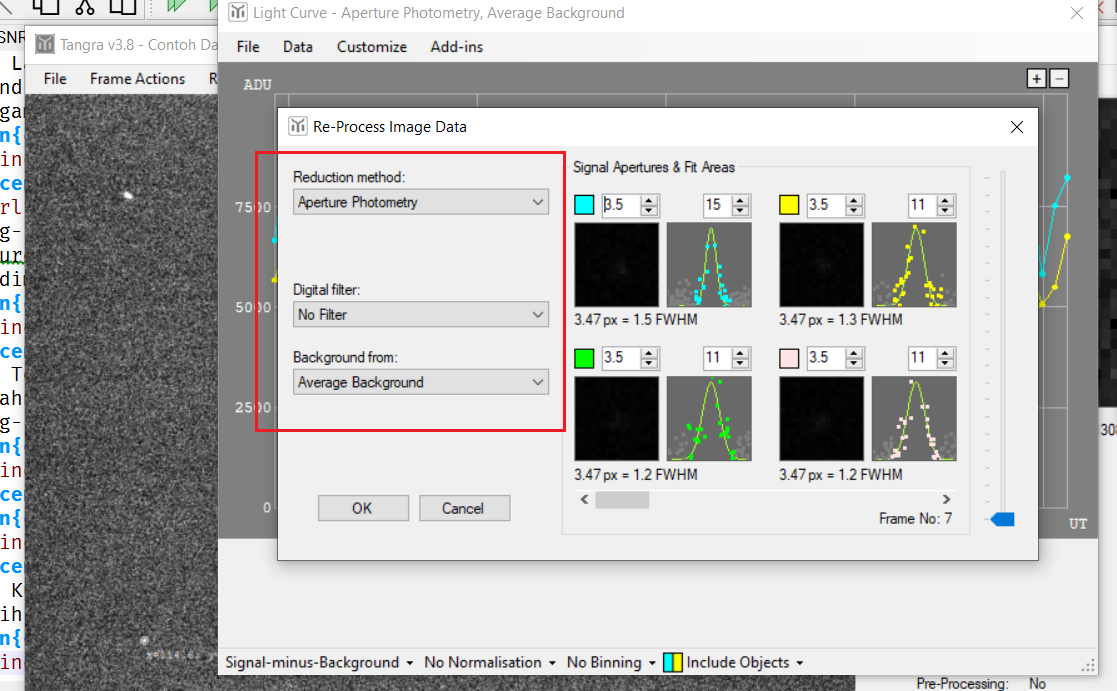
\includegraphics[width=0.5\linewidth]{tangra-reprocess-pilihan}
	\end{center}
	\item Lakukan pemeriksaan kualitas cepat sebelum ekspor: cek tidak ada saturasi pada target/pembanding, cek aperture tetap mengikuti bintang (tidak \textit{drift}), dan cek tidak ada \textit{outlier} ekstrem yang jelas tidak fisis.
	\item Jika hasil sudah sesuai, ekspor ke file .csv untuk pengolahan lebih lanjut (dengan AOTA atau program lain) atau pilih \textit{File > Save Light Curve} untuk menyimpan ke file .lc untuk analisis dengan AOTA.
	\underline{Catatan:} sebelum ekspor final, verifikasi kembali metadata waktu (UTC, \textit{cadence}/durasi paparan, dan indikasi \textit{dropped frame} jika ada) agar analisis kejadian okultasi tetap akurat.
	\begin{center}
		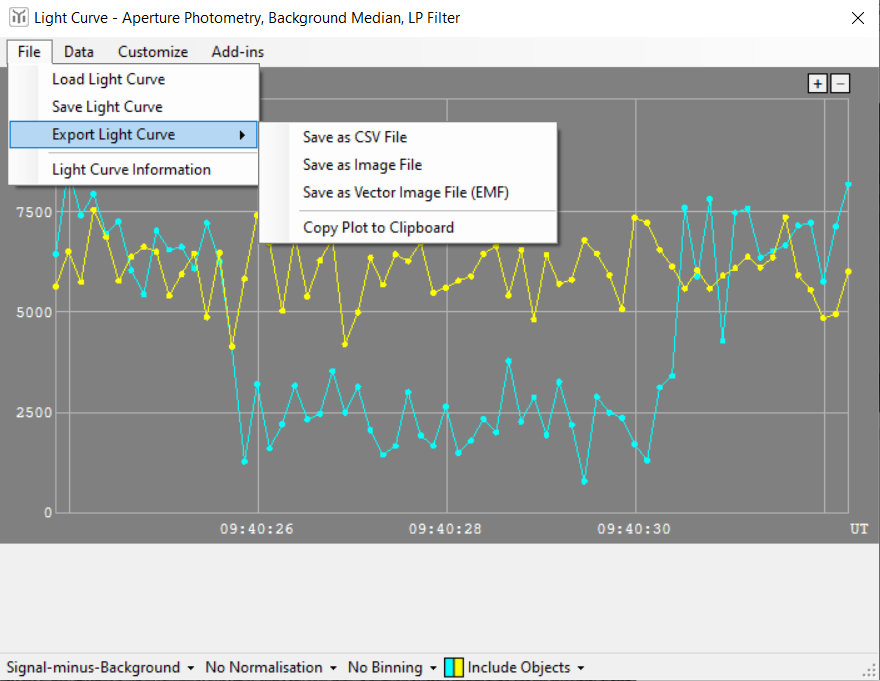
\includegraphics[width=0.5\linewidth]{tangra-export}
	\end{center}
\end{enumerate}
\end{document}